\documentclass[conference]{IEEEtran}
\IEEEoverridecommandlockouts
% The preceding line is only needed to identify funding in the first footnote. If that is unneeded, please comment it out.
\usepackage{cite}
\usepackage{amsmath,amssymb,amsfonts}
\usepackage{algorithmic}
\usepackage{graphicx}
\usepackage{textcomp}
\usepackage{xcolor}
\usepackage{soul}
\usepackage{biblatex} %Imports biblatex package
\addbibresource{bibliography.bib} %Import the bibliography file
\def\BibTeX{{\rm B\kern-.05em{\sc i\kern-.025em b}\kern-.08em
    T\kern-.1667em\lower.7ex\hbox{E}\kern-.125emX}}
    
    
\begin{document}


\title{Semantic Segmentation on Satellite Imagery (must change*)\\}
\author{\IEEEauthorblockN{Nancy Nigam}
\IEEEauthorblockA{\textit{Computer Science} \\
\textit{CIMS, NYU}\\
New York City, US\\
nn2163@nyu.edu}
\and
\IEEEauthorblockN{Jorge Roldan}
\IEEEauthorblockA{\textit{Computer Science} \\
\textit{CIMS, NYU}\\
New York City, US\\
jlr9718@nyu.edu}
\and
\IEEEauthorblockN{Aditya Upadhyaya}
\IEEEauthorblockA{\textit{Computer Science} \\
\textit{CIMS, NYU}\\
New York City, US\\
au2056@nyu.edu}
}
\maketitle

% \begin{abstract}
% \hl{Do abstract when we are done with everything else}
% \end{abstract}

% ============================
\section{Introduction}
% ============================
The evolution of remote sensing technologies over the last couple of decades has drastically increase the amount of satellite imagery datasets available and open to the public. The increase of data available plus the advances in the fields of Machine Learning and Computer Vision to study and gain insights from these datasets has open the door to opportunities to tackle new type of problems at scale. \\ \indent
One of these opportunities is the ability to manage and survey the properties of different land covers all around the world by automating the identification of terrains, natural or artificial structures, or any other object of interest using semantic segmentation models. These models receive as an input a source image and a mask where each pixel indicates the class of that pixel in the source image. Once the model is trained, it will ideally be able to predict a mask for a new, unseen image.  \\ \indent
Automatic classification at the pixel level of satellite imagery can then play a key role at monitoring, managing, and detecting changes on land covers. This is directly related to the Life on Land objective from the United Nation's Sustainable development goals  \cite{united_nations}, which deals with protecting, restoring and promoting sustainable use of terrestrial ecosystems. Leveraging Machine Learning models for semantic segmentation tasks on these large satellite imagery datasets is a promising approach for successfully accomplish this sustainability goal.

% ============================
\section{Related Work}
% ============================
The application of semantic segmentation models on satellite imagery have been shown to perform well in many cases \cite{DBLP:journals/corr/abs-2003-02899}\cite{DBLP:journals/corr/abs-2010-06285}\cite{DBLP:journals/corr/abs-1911-12903}\cite{Avenash2019SemanticSO}\cite{9137717}\cite{DBLP:journals/corr/BadrinarayananK15}\cite{DBLP:journals/corr/abs-1711-08681}\cite{DBLP:journals/corr/abs-1904-03983}\cite{DBLP:journals/corr/abs-1902-04604}.
Authors in \cite{DBLP:journals/corr/abs-2003-02899} trained a ResNet model architecture for classification on the BigEarthNet dataset \cite{DBLP:journals/corr/abs-1902-06148}. They also trained a modified U-Net architecture for the segmentation tasks using a customized dataset, which combined a CORINE Land Cover map as well as Sentinel-2 source images. Using these combinations of architectures and datasets, they obtained an overall F1 score of 0.749 for the classifier with 43 possible classes, as well as a high IoU score for the segmentation model. \\ \indent
Authors in other works such as \cite{DBLP:journals/corr/abs-2010-06285} used a pretrained ResNet50 and transfer it into a U-Res-Net for classification tasks. They also used a customized version of U-Net for the segmentation tasks. A common technique in these works is to use data  augmentation to overcome the challenge of small size of the satellite imagery datasets currently available.  \\ \indent
Other interesting applications of semantic segmentation models is to detect changes in different land covers terrains over time as done in \cite{DBLP:journals/corr/abs-1911-12903}. In this work, the authors use Deeplab v3+  \cite{DBLP:journals/corr/ChenPSA17} and build a complete training pipeline to create a land cover change detection system achievin a mean IoU of 0.756.




% ============================
\section{Datasets}
% ============================
% ----------------------------------------
\subsection{LandCoverNet Dataset}
% ----------------------------------------
\subsubsection{Dataset Characteristics}
The LandCoverNet dataset consists of 1980 image chips with a resolution of (256px x 256px) where each image chip correspond to a specific location across Africa. For each image chip there are several source images at different time stamps during 2018  obtained from the Sentinel-2 Surface reflectance product (L2A). Furthermore, each image has a corresponding mask with the labels for each pixel as shown in table \ref{landcovernet_dataset} \cite{DBLP:journals/corr/abs-2012-03111}. 





\begin{table}[htbp]
\centering
\caption{LandCoverNet dataset}
\begin{tabular}{|p{1.8cm}|p{0.6cm}|p{1.6cm}|}
 \hline
 \multicolumn{3}{|c|}{\textbf{LandCoverNet Dataset Classes}} \\
 \hline
 \textbf{Class Name} & \textbf{Pixel Value}& \textbf{RGB Value} \\
 \hline
 Unkown & 0  & (0,0,0)\\ 
 \hline
 Water & 1  & (0,0,255)\\ 
 \hline
 Artificial & 2  & (136,136,136)\\ 
 \hline
 Natural & 3  & (209,164,109)\\ 
 \hline
 Snow/ice & 4 &  (245,245,255)\\ 
 \hline
 Wooddy & 5  & (214,76,43)\\ 
 \hline
 Cultivated & 7  & (24, 104, 24)\\ 
 \hline
 (Semi) Natural & 7  & (0, 255, 0)\\ 
 \hline
\end{tabular}
\label{landcovernet_dataset}
\end{table}

\subsubsection{Data collection, preprocessing, and challenges}

The LandCoverNet dataset \cite{DBLP:journals/corr/abs-2012-03111} was collected using the Radiant MLHub API, \cite{radiant_mlhub_api}. Since this API is in the early stages of development, we faced many issues while collecting the data. The primary issue was that we couldn't filter out source images with clouds on it, therefore a significant portion of the dataset had source images with clouds. \\ \indent
The format of the sources and mask images was TIF, therefore we had to convert all of these images into PNG by stacking the Red Blue, and Green channels. The masks also had initially the TIF format with one channel, where the value of each pixel represents the class from table \ref{landcovernet_dataset}. Finally, we used the RGB mapping to convert each mask to an RGB PNG image. The scripts we created to do this are provided in the data$\_$preprocessing folder in the source code.


\subsection{Semantic Segmentation of Crop Type in Ghana Dataset}
\subsubsection{Dataset Characteristics}
The Crop Type in Ghana dataset \cite{Rustowicz2019SemanticSO} consists of images from Sentinel-1 and sentinel-2 from Ghana and South Sudan taken over 2016 and 2017. For each image chip, there are several source images at different time stamps, and a corresponding mask. There are 25 labels for different type of crops as shown in table \ref{ghana_dataset_class_table}.  


\begin{table}[htbp]
\centering
\caption{Ghana Dataset}
\begin{tabular}{|p{2.2cm}|p{0.7cm}|p{1.6cm}|}
 \hline
 \multicolumn{3}{|c|}{\textbf{Crop Type in Ghana Dataset Classes}} \\
 \hline
 \textbf{Class Name} & \textbf{Pixel Value}& \textbf{RGB Value} \\
 \hline
  Unknown & 0  &  (0, 0, 0)\\ 
 \hline
  Ground nut & 1  & (80,0,165) \\ 
 \hline
  Maize & 2  & (255,204,0) \\ 
 \hline
  Rice & 3  & (0,244,244)\\ 
 \hline
  Soya bean & 4  & (105,105,105)\\ 
 \hline
  Yam & 5  & (255,255,102) \\ 
 \hline
  Intercrop & 6  & (255,153,153)\\ 
 \hline
  Sorghum & 7  & (127,222,209)\\ 
 \hline
  Okra & 8  & (222,127,219)\\ 
 \hline
  Cassava & 9  & (108,67,107)\\ 
 \hline
  Millet & 10  & (152,134,94)\\ 
 \hline
  Tomato & 11 & (99,228,150) \\ 
 \hline
  Cowpea & 12  & (99,176,228)\\ 
 \hline
  Sweet Potato & 13 & (255,186,186)\\ 
 \hline
  Babala Beans & 14  & (204,0,102) \\ 
 \hline
  Salad Vegetables & 15  & (102,51,0)\\ 
 \hline
  Bra and Ayolo  & 16  & (204,204,255)\\ 
 \hline
  Watermelon & 17  & (0,102,204)\\ 
 \hline
  Zabla & 18 & (255,0,255)\\ 
 \hline
  Nili & 19 & (102,0,204)\\ 
 \hline
  Kpalika & 20 & (141,51,117)\\ 
 \hline
  Cotton & 21 & (145,187,192)\\ 
 \hline
  Akata & 22 & (155,123,219)\\ 
 \hline
  Nyenabe & 23 & (193,0,76)\\ 
 \hline
  Pepper & 24 & (204,255,153)\\ 
 \hline
\end{tabular}
\label{ghana_dataset_class_table}
\end{table}


\subsubsection{Data collection, preprocessing, and challenges}
The Ghana dataset was collected using the Radiant MLHub API \cite{radiant_mlhub_api}.
One major advantage of this dataset is that it provides a cloud mask for each source image, which was not the case for the LandCoverNet dataset. We used this cloud mask in order to filter out any images that had clouds on it. We also converted all the source and masks images from TIF to PNG format. We have include these scripts in the data$\_$preprocessing folder in the source code. A major drawback of this dataset is that the resolution of the images is just (64px x 64px), which is rather low to successfully train models for semantic segmentation.


\subsection{LandCover.ai Dataset}



\subsubsection{Dataset Characteristics}
The LandCover.ai dataset consists of satellite imagery for semantic segmentation applications covering a region of Poland of a total area of 216.2 km$^2$ \cite{DBLP:journals/corr/abs-2005-02264}. The original dataset consists of 41 orthophoto tiles of 5 km$^2$ where 33 images and 8 images have a resolution of (9000 px x 9500 px) and (4200 px x 4700 px), respectively. \\ \indent
The authors of this dataset \cite{DBLP:journals/corr/abs-2005-02264} provided a script which we used to split these 41 images and their respective masks into 10,674 source and 10,674 masks images of (512 px x 512 px) resolution. The land cover of these images consist of agricultural areas (60 \%) and mixed forests (29.6 \%). \\ \indent



\subsubsection{Classes and RGB Mapping}
The name of the classes, their respective pixel value, and RGB value are shown in table \ref{landcover_ai_classes}. The annotations were made manually by the authors using VGG  Image Annotator (VIA) \cite{dutta2019vgg}. According to \cite{DBLP:journals/corr/abs-2005-02264}, there are 12280 buildings (1.85 km$^2$), 72.02 km$^2$ of woodland, 13.15 km$^2$ of water, 3.5 km$^2$ of roads, and 125.75 km$^2$ of background, that is, the unknown class. \\

\begin{table}[htbp]
\centering
\caption{LandCover.ai Dataset}
\begin{tabular}{|p{1.2cm}|p{0.7cm}|p{1.6cm}|}
 \hline
 \multicolumn{3}{|c|}{\textbf{Landcover.ai Dataset Classes}} \\
 \hline
 \textbf{Class Name} & \textbf{Pixel Value}& \textbf{RGB Value} \\
 \hline
 Unknown & 0  & (0,0,0)\\ 
 \hline
 Building & 1  & (80,0,165)\\ 
 \hline
 Woodland & 2  & (255,204,0)\\ 
 \hline
 Water & 3  & (0,244,244)\\ 
 \hline
 Road & 4  & (105,105,105)\\ 
 \hline
\end{tabular}
\label{landcover_ai_classes}
\end{table}
\\

\subsubsection{Data collection, preprocessing, and challenges}
The source images and masks are LandCover.ai were originally provided in PNG and JPG format, respectively. The masks consisted of one channel where each pixel had the value of the class (0 - 4) as shown in table \ref{landcover_ai_classes}. In order to be able to use them in our model, we mapped each pixel value to the corresponding RGB value and generated a new PNG mask that can directly be used when training our model. This python script can be found in the data$\_$preprocessing folder in our source code. \\ \indent
Two major advantages of the Landcover.ai dataset, compared the LandCoverNet and Crop Type in Ghana dataset is that the source images  in Landcover.ai did not contain clouds since the authors \cite{DBLP:journals/corr/abs-2005-02264} filtered out any of these images. Furthermore, the high-resolution and quality of the images makes this dataset the ideal one to train our semantic segmentation models.      



% ============================
\section{Methodology}
% ============================
% ----------------------------------------
\subsection{Architectures}

For the purpose of our experiments, we leverage a U-Net network \cite{ronneberger2015unet}. U-Net is a fully convolution neural network used extensively for image segmentation. It involves encoder and decoder components connected with skip connections. For the classification model that serves as our encoder and extracts features of different spatial resolution, we use a ResNet architecture \cite{DBLP:journals/corr/HeZRS15}. As part of our ablation study, we also review a U-Net++ network \cite{DBLP:journals/corr/abs-1807-10165} which consists of convolution layers on skip pathways.
% ----------------------------------------

% ----------------------------------------
\subsection{Evaluation Metrics}
% ----------------------------------------
 The lead evaluation metric for us is the Jaccard Index, also known as Intersection over Union (IoU).
\begin{equation*}
    IoU=\frac{target \cap prediction}{target \cup prediction}
\end{equation*}

In addition to IoU, we also capture Pixel Accuracy, Precision, and Recall. High pixel accuracy (the number of pixels classified correctly) doesn't always imply good segmentation results, especially in cases of class imbalance. This is true in our case since the 'woodland' class dominates all other classes.

% ============================
\section{Setup and Experiments}
% ============================

\subsection{Setup}
Our entire data augmentation, training, and prediction pipeline is implemented on the PyTorch framework and we use the NVIDIA V100 GPU to speed up our computations. The SMP library \cite{Yakubovskiy:2019} provides us segmentation models with pre-trained backbones. 
\\
\\Typically, neural network initialized with weights from a pre-trained network shows better performance and for our purposes, we initialize our ResNet encoder with ImageNet weights. The encoder depth is kept at a constant value of 5 throughout the scope of our experiments. 

\subsection{Hyperparameters}
Our seed dataset is divided into train-validation-test with a ratio of 80:10:10. A batch size of 32 works best for our use-case and we keep this value constant throughout. The Adam optimizer is our choice for all our experiments as it helps us converge faster and we apply a softmax activation after the final convolution layer. A bit of fine-tuning helps us arrive at a starting learning rate of $1\text{e-}4$ for our StepLR with a multiplicative factor of 0.1 every 15 epochs. The step size varies when it comes to training with the ResNet101 encoder. Finally, the choice for our loss function is the Focal Loss as it helps us address class imbalance. We do consider other loss functions (Cross Entropy Loss and Dice Loss) and we discuss this in detail in the next section.
\subsection{Experiments}
We conduct a variety of experiments across multiple configurations of our pipeline and we discuss them in detail.

\subsubsection{Dataset Challenges}
Datasets in their raw form pose a serious challenge due to multiple factors. For instance, the Ghana Dataset \cite{Rustowicz2019SemanticSO} comprises of low-res images, class imbalance, and high cloud cover. On the other hand, the LandCoverNet dataset excels in terms of image quality and adequate labels for each class, but it comes up short when it comes to cloud cover. Figure 1 illustrates the results of one such experiment we conduct on this dataset.

\subsubsection{Loss Functions} The choice of loss function plays a major role for any architecture as it dictates our learning process. In an effort to gain a deeper understanding of the impact of our choices, we do a comparative analysis of three popular loss functions - Focal, Dice, and Cross Entropy. To keep all other parameters constant, We plug a ResNet18 encoder (with pre-trained ImageNet weights) in our U-Net network. Training is done for a total of 40 epochs. We keep our initial dataset as the baseline (Fig1) and capture the results when we intentionally skew the dataset heavily towards one of the classes (woodland) (Fig x \hl{Fix figure number}). Fig 1 depicts the progression of IoU over the iterations when the dataset isn't imbalanced.
\usepackage{float}

\begin{figure}[!h]
    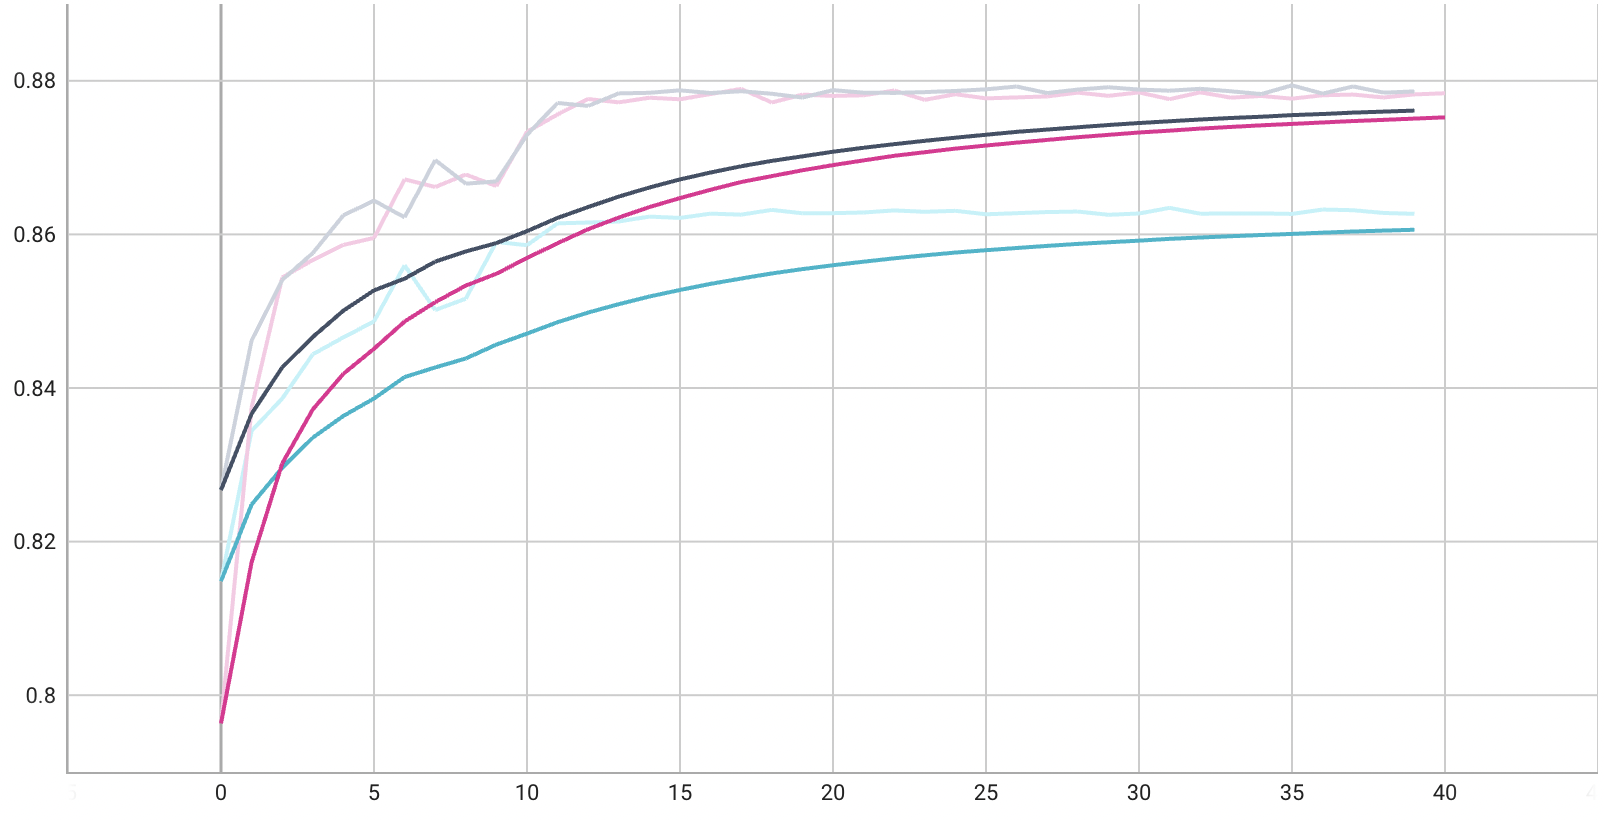
\includegraphics[width=9cm, height=5cm]{images/roads-losses/three-losses-iou.png}
    \caption{\hl{Mention dataset used} Progression of IoU Scores over 40 epochs for Focal Loss (Magenta), Dice Loss (Teal), and Cross Entropy Loss (Gray). U-Net network having a ResNet18 encoder pre-trained with ImageNet weights. The dataset doesn't have an imbalance. }
\end{figure}


\subsubsection{Network and Encoders} With an intent to observe the effect of the depth of network, we try multiple encoders (ResNet18, ResNet34, and ResNet101) for our U-Net network. Additionally, we evaluate a U-Net++ network (using a ResNet34 encoder). All encoders are initialised with ImageNet weights. We train for a total of 40 epochs and employ Focal Loss as our loss function. The visualization results are shown in Fig 1. Fig 2,3,4 consist of graphs depicting the progession of metrics.

\begin{figure}[!h]
    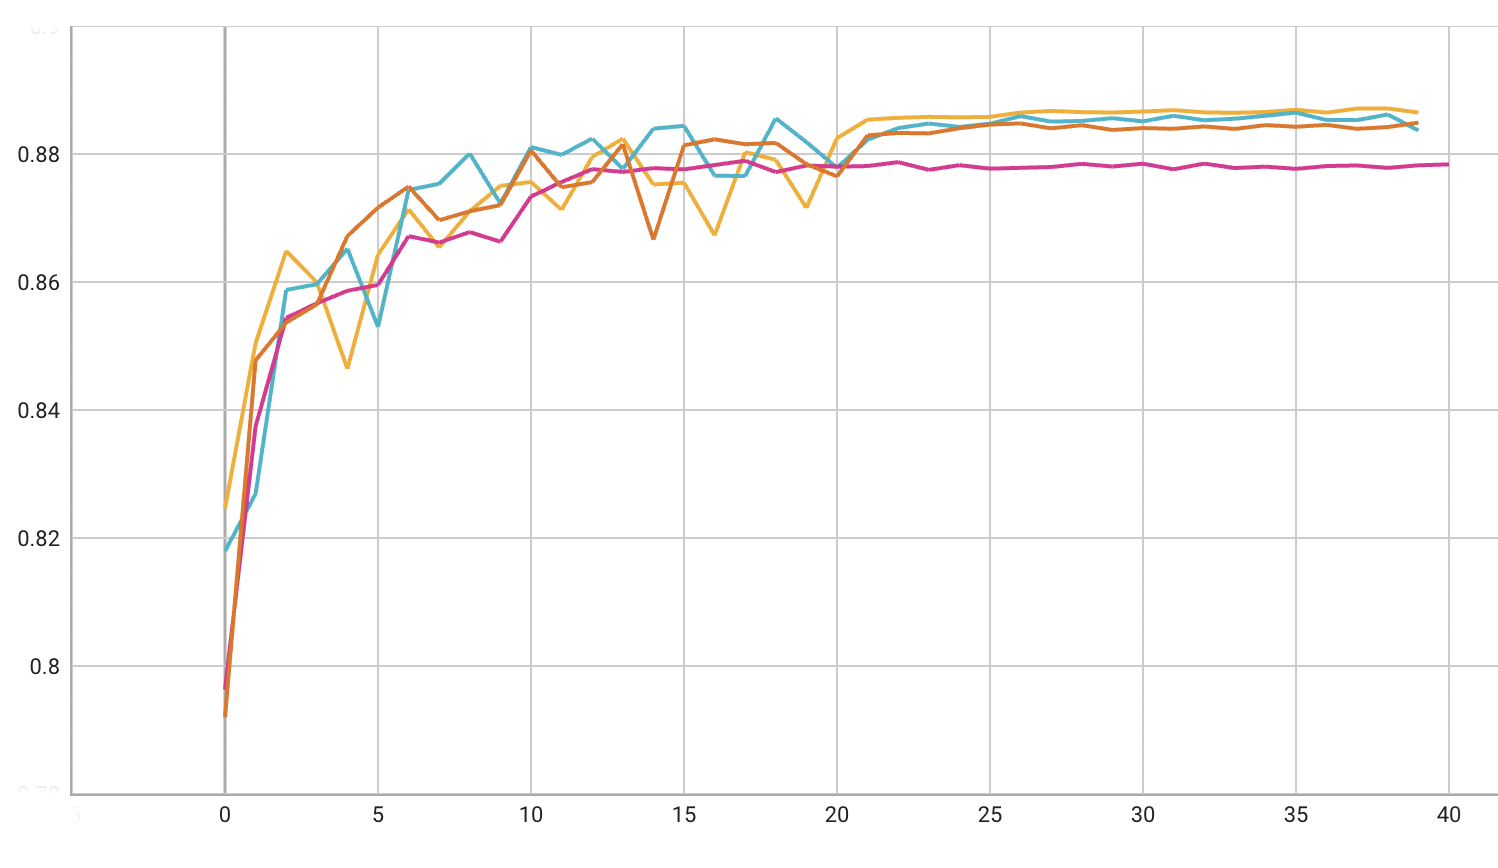
\includegraphics[width=9cm, height=5cm]{images/encoders/encoders_iou.png}
    \caption{\hl{Mention dataset used} Progression of IoU Scores over 40 epochs for U-Net ResNet18 (Pink), U-Net ResNet34 (Orange), U-Net ResNet101 (Blue), and U-Net++ ResNet34 (Yellow). Focal Loss is being employed and all encoders are initialized with pre-trained Image-Net weights.}
\end{figure}


% \begin{figure}[h]
%     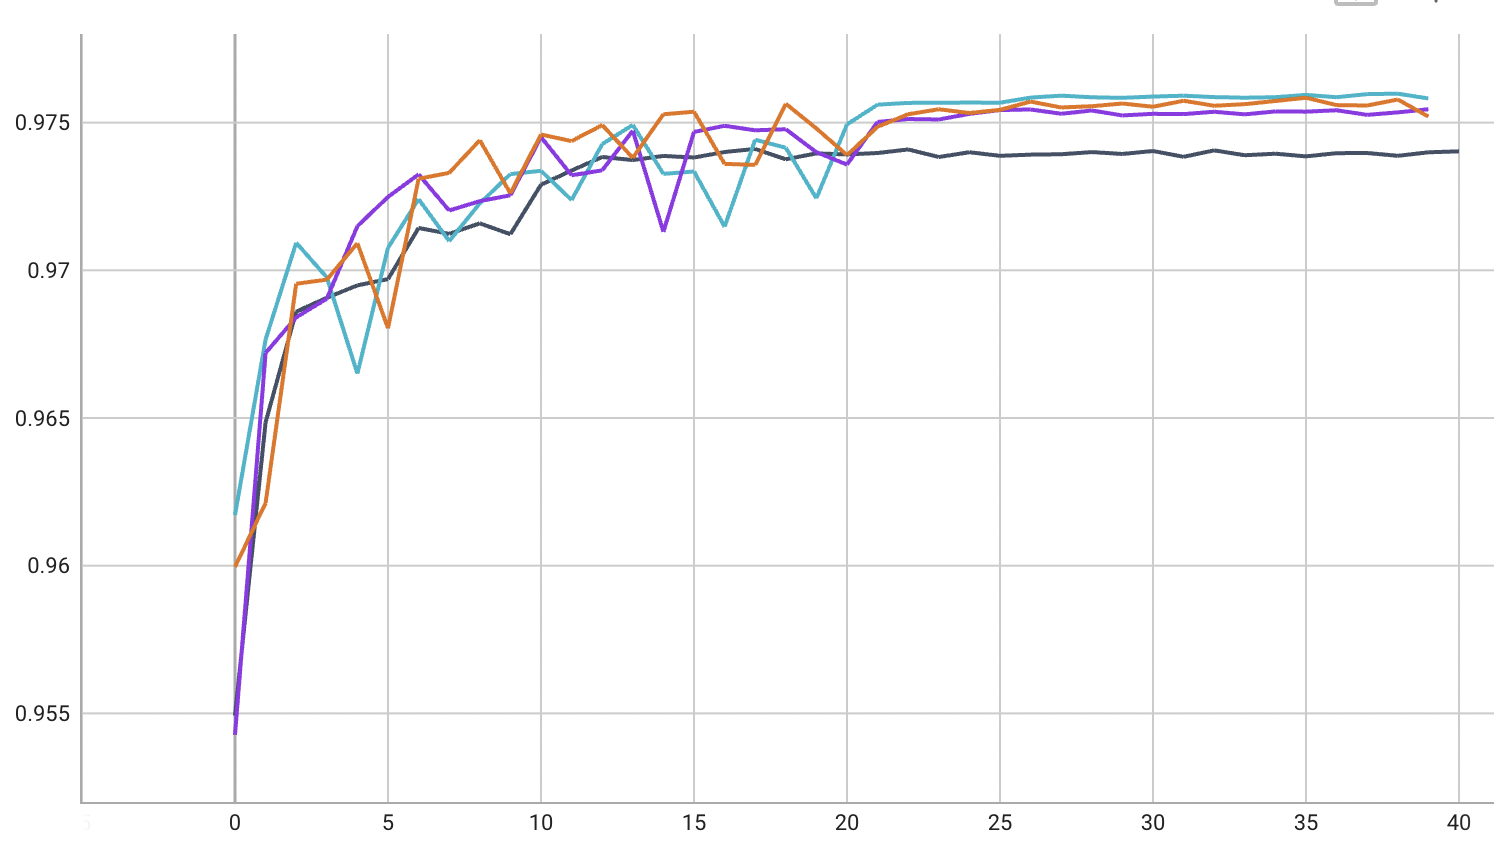
\includegraphics[width=9cm, height=5cm]{images/encoders/encoders_accuracy.png}
%     \caption{Progression of Pixel Accuracy over 40 epochs for U-Net ResNet18 (Dark Gray), U-Net ResNet34 (Purple), U-Net ResNet101 (Orange), and U-Net++ ResNet34 (Sky Blue). Focal Loss is being employed and all encoders are initialized with pre-trained Image-Net weights.}
% \end{figure}

\begin{figure}[!h]
    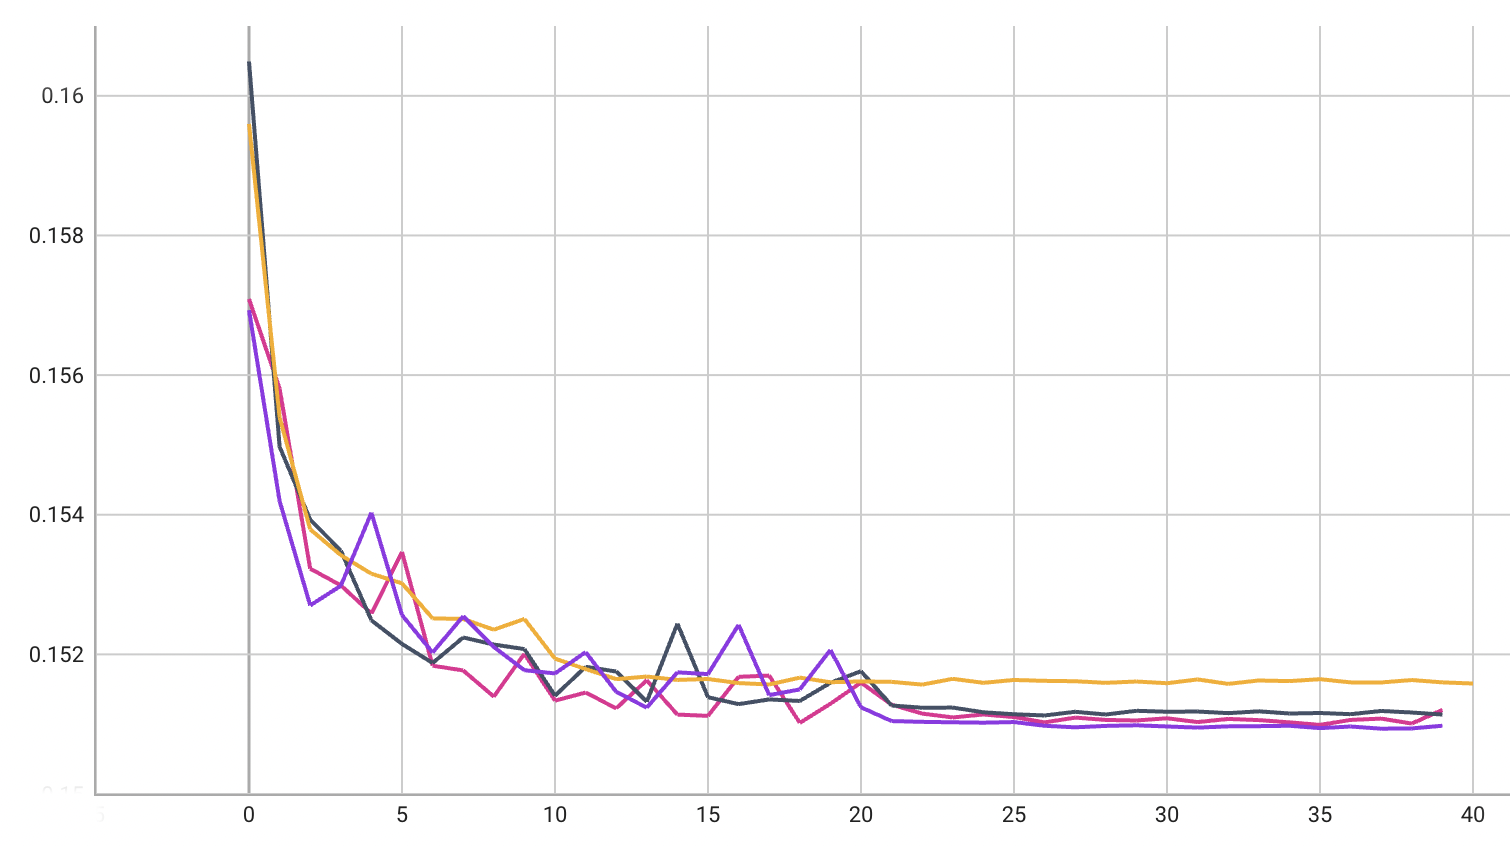
\includegraphics[width=9cm, height=5cm]{images/encoders/encoders_focalloss.png}
    \caption{\hl{Mention dataset used}  Progression of Focal Loss values over 40 epochs for U-Net ResNet18 (Yellow), U-Net ResNet34 (Dark Gray), U-Net ResNet101 (Pink), and U-Net++ ResNet34 (Purple).}
\end{figure}

\begin{figure}[!h]
    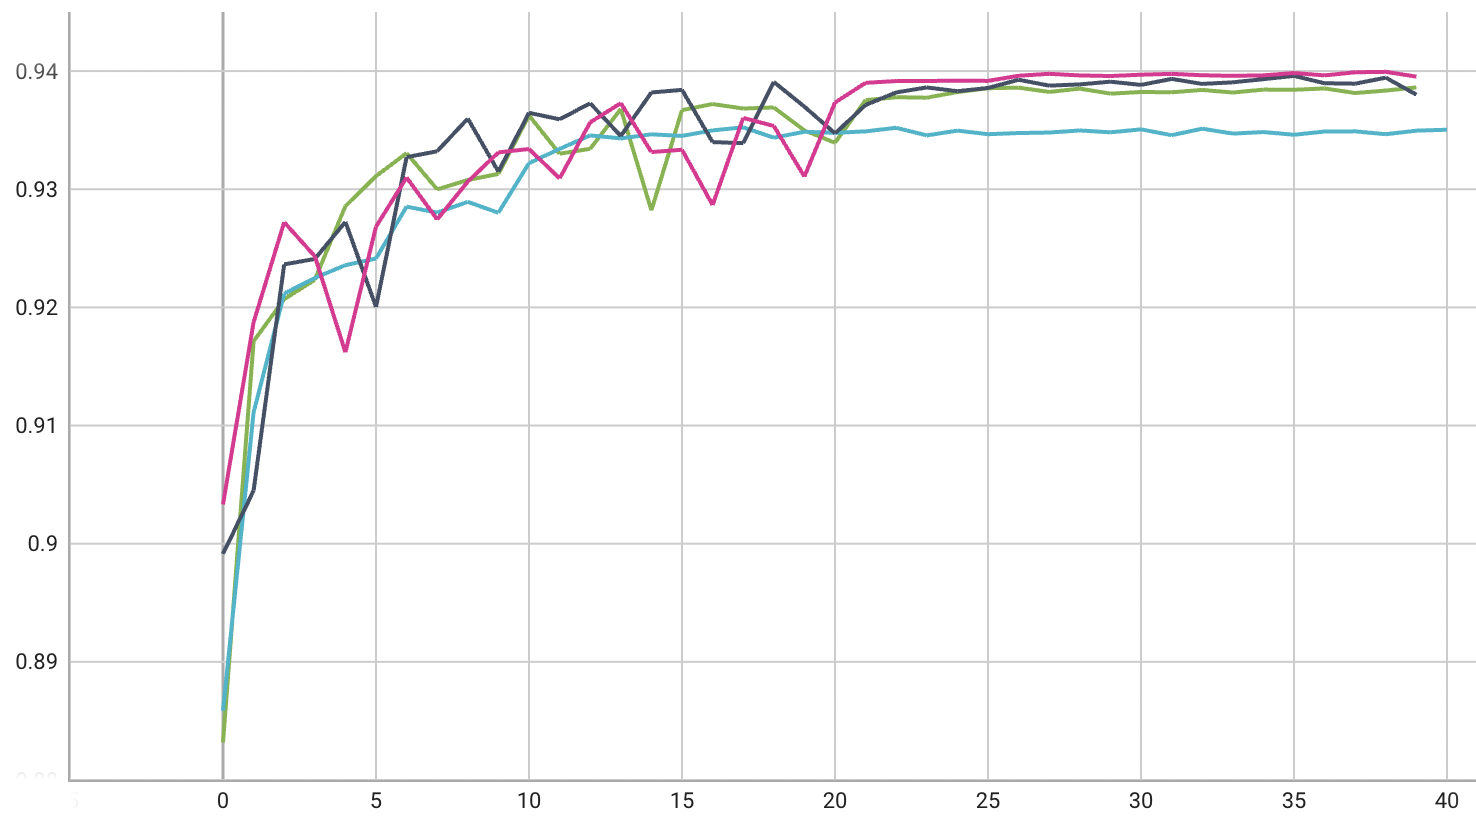
\includegraphics[width=9cm, height=5cm]{images/encoders/encoders_fscore.png}
    \caption{\hl{Mention dataset used} Progression of F Scores over 40 epochs for U-Net ResNet18 (Blue), U-Net ResNet34 (Green), U-Net ResNet101 (Gray), and U-Net++ ResNet34 (Pink). }
\end{figure}


% ============================
\section{Results}
% ============================
\begin{figure*}
    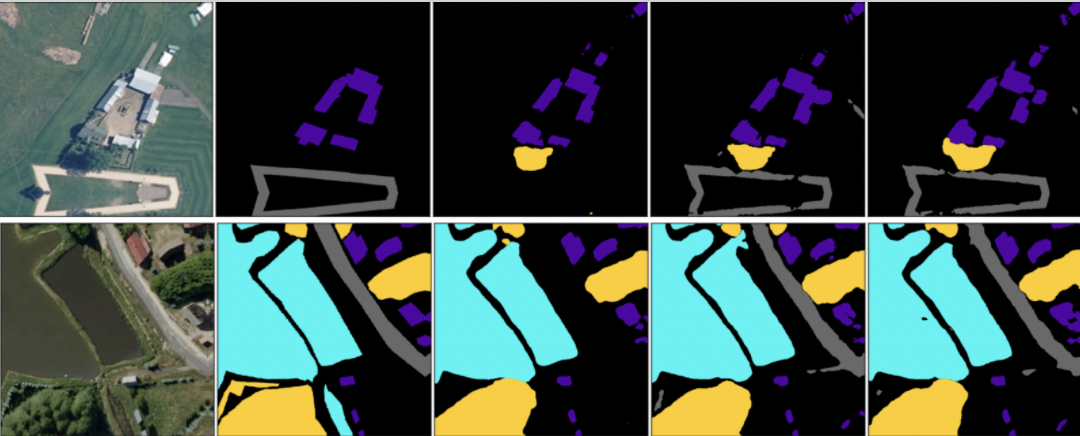
\includegraphics[]{images/no-roads-losses/no-roads-smaller.png}
    \caption{\hl{Mention dataset used} Prediction on a highly-imbalanced dataset with a U-Net network on a ResNet18 encoder. The first column contains the actual images, the second column represents the target mask, the third, fourth, and fifth columns represent the predicted mask with Dice, Focal, and Cross Entropy Loss respectively. Dice Loss(third columns) fails to detect the minority class (roads) in a lot of samples}
\end{figure*}

\begin{figure*}
    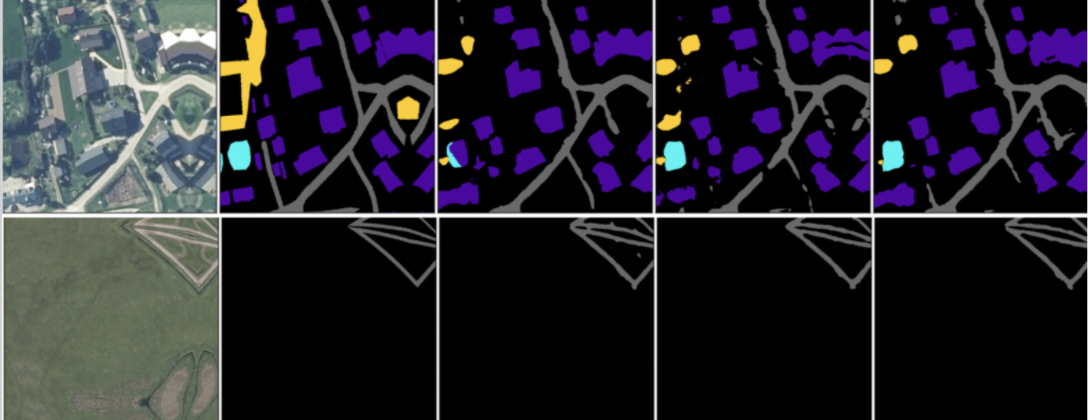
\includegraphics[]{images/roads-losses/roads-smaller.png}
    \caption{\hl{Mention dataset used} Prediction on a more balanced dataset with a U-Net network on a ResNet18 encoder. The first column contains the actual images, the second column represents the target mask, the third, fourth, and fitth columns represent the Predicted Mask with Dice, Focal, and Cross Entropy Loss respectively}
\end{figure*}

\begin{figure*}
    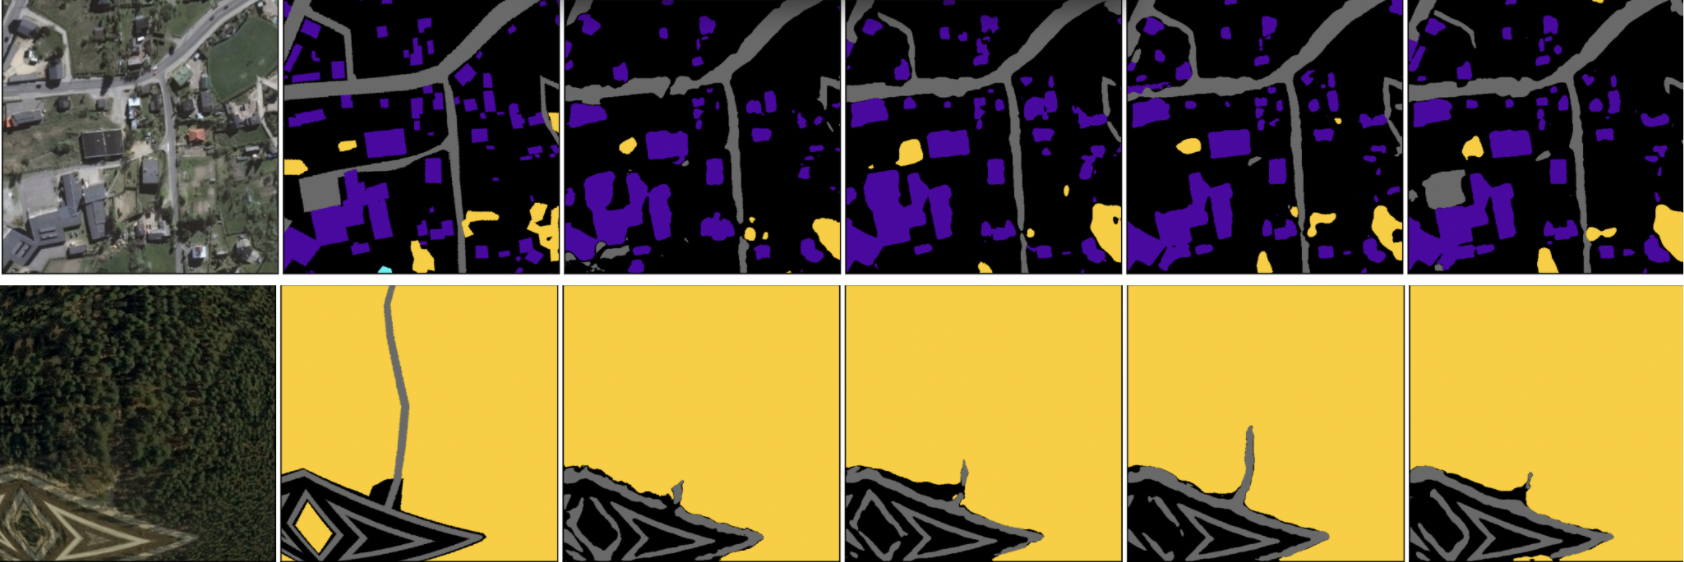
\includegraphics[width=\textwidth]{images/encoders/encoders-vis.png}
    \caption{\hl{Mention dataset used} Prediction on a more balanced dataset with a U-Net network on a ResNet18 encoder. The first column contains the actual images, the second column represents the target mask, the third, fourth, and fitth columns represent the Predicted Mask with Dice, Focal, and Cross Entropy Loss respectively}
\end{figure*}
\begin{enumerate}
    \item \hl{Specify that these results are for only the Landcover.ai dataset?} 
    \item Roads and Buildings pose a challenge owing to their minority representation and narrowness (in case of roads). A lot of samples also present with scenarios where the road network is hidden under a canopy of trees.
    \item Dice Loss consistently misses out on the minority classes in cases of severe imbalance. This is shown best in Fig x where it fails to detect Roads.
    \item Focal Loss performs marginally better (mean IoU = 0.875 on validation set) than both Dice and Cross Entropy when the dataset is slightly balanced. However, the difference is stark in cases of severe imbalance.
    \item When it comes to the number of layers in our encoder, we observe that depth matters and ResNet18 consistently achieves a 1 point lower mean IoU score (0.871) on the validation set when compared to the other encoders over the course of 40 epochs.
    \item ResNet101 on a U-Net network achieves a mean IoU score of 0.886 on the validation set and a visual inspection of the results hint towards it being able to detect shapes concretely.
    \item The combination of U-Net++ and ResNet34 performs only slightly better (mean IoU = 0.8871) than that U-Net and ResNet34 (mean IoU = 0.8843).
\end{enumerate}

% ============================
\section{Conclusion}

In this study, we present a data processing and training pipeline that can be used to automate Satellite Imagery segmentation. Semantic Segmentation has a myriad of applications ranging from disaster resilience to tracking regional urbanization, environmental monitoring, and the Sentinel-2 mission has made this data readily available. We discuss the challenges that one can face while working on a new dataset, ways to overcome them, and create reliable images and masks for training. We then conduct a series of experiments to gauge the importance of choosing a loss function. Loss functions are a critical component of any learning-based approach and one of the factors that should govern this choice is the extent of class imbalance. We also observe the effects of the depth of an encoder by exploring different flavors of a U-Net network. Finally, the best performing model is the U-Net using a ResNet101 achieving an \hl{Should be IoU instead of mIoU?} mIoU score of 0.88. In the future, we can extend this study to track changes in a particular landscape over a period of time.
% ============================



\begin{figure}[h]
    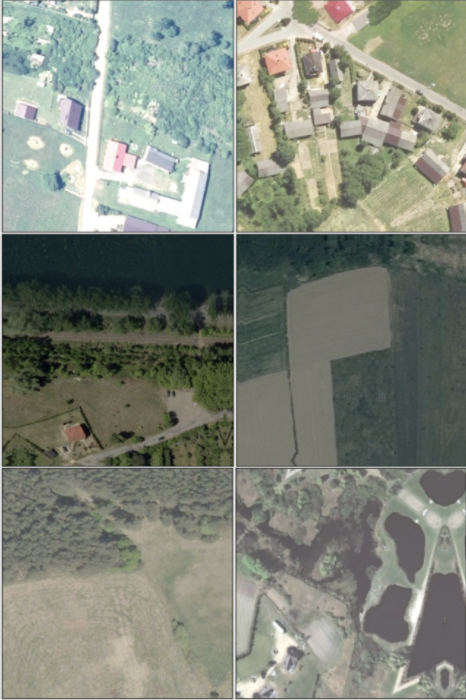
\includegraphics[width=6cm, height=8cm]{images/dataset-vis.png}
    \caption{\hl{Mention dataset used, please place this in the correct place} Seed Dataset}
\end{figure}



\newpage
\printbibliography %Prints bibliography


\end{document}

